\documentclass{article}

% Language setting
% Replace `english' with e.g. `spanish' to change the document language
\usepackage[english]{babel}

\usepackage{booktabs}
\usepackage{threeparttable}
\usepackage{siunitx} % For decimal alignment
% Set page size and margins
% Replace `letterpaper' with `a4paper' for UK/EU standard size
\usepackage[letterpaper,top=2cm,bottom=2cm,left=3cm,right=3cm,marginparwidth=1.75cm]{geometry}

% Useful packages
\usepackage{amsmath}
\usepackage{graphicx}
\usepackage{enumitem}
\usepackage[colorlinks=true, allcolors=blue]{hyperref}
\usepackage{booktabs}
\usepackage{float} % for [H]
\usepackage{graphicx}
\usepackage{caption}
\usepackage{comment}
\usepackage{subcaption}
\usepackage{array}
\usepackage{subcaption}


\title{GEO1016 - Assignment 2 : Triangulation}
\author{Job Segers (6597084), Niranjan Pradeep (6401643), Akhil Veeranki (6305105)}



\begin{document}

\maketitle

\section{Methodology}
\subsection{Recovering relative camera pose}
In this report the goal is to recover 3D structure from two images taken from different viewpoints using corresponding points in these images. The intrinsic camera parameters, and thus the camera matrix $K$, are assumed to be known and the same for both pictures.

To begin we wish to recover the relative rotation $R$ and translation $\mathbf{t}$ of the second picture from the first. This is done through first estimating the fundamental matrix $F$ with the normalized eight point algorithm. Given our corresponding points $\mathbf{p}_i $ and $\mathbf{p}_i'$, we first normalize them by translating towards the mean and then scaling so that the average distance from the mean is $\sqrt{2}$, yielding: 
\[
\mathbf{q}_i = T\mathbf{p}_i \hspace{4cm} \mathbf{q}_i' = T'\mathbf{p}_i'
\]
%Note i use A instead of W here, W is a different matrix later
We then utilize the epipolar constraint $\mathbf{q}_i'^TF_q\mathbf{q_i} = 0$ to set up a system of linear equations, then written as $A\mathbf{f}=0$, where $A$ is an $n \geq 8$ by $9$ matrix derived from the coordinates of the correspondences and $\mathbf{f}$ are the values of the fundamental matrix. This is then solved for in a least squares manner using Singular Value Decomposition (SVD) to obtain $\hat{F}_q$, which is an estimate that may have full rank. To obtain a matrix obeying the rank 2 constraint on the fundamental matrix we once again use SVD. 
\[
F_q = U\begin{pmatrix}
    d_1 & 0 & 0 \\
    0 & d_2 & 0 \\
    0 & 0 & 0
\end{pmatrix}V^T
\]
Here $d_1$ and $d_2$ are the largest singular values of $\hat{F}_q = UDV^T$. We then denormalize through $F = T'^TF_qT$. We then obtain the camera Essential matrix $E = [\mathbf{t}_\times]R$ from this through $E = K^TFK$.

From the SVD of the essential matrix we can then obtain $R$ and $\mathbf{t}$ as
\begin{gather*}
    R = \det(UWV^T)UWV^T \quad \mathrm{or} \quad R= \det(UW^TV^T)UW^TV^T \\ 
    \mathbf{t} = \pm \mathbf{u}_3
\end{gather*}
Where $\mathbf{u}_3$ is the third column of $U$ and $W$ is a 3 by 3 matrix with $W_{12} = 1$, $W_{21}=-1$ and $W_{33}=1$, and all other values zero. With two options for both $R$ and $\mathbf{t}$ we get four possible combinations. The correct orientation has a positive $z$-value for the observed points in both camera coordinate frames, which can be checked for after estimation of the points' locations with all four options.

We thus calculate the four options for $M' = K [R\quad \mathbf{t}]$, and define $M = K[I\quad 0]$ We then derive a linear equation to for the triangulation from the restraints resulting from $M\mathbf{P}= \mathbf{p}$ and $M'\mathbf{P} = \mathbf{p}'$. This yields:
\[ A\mathbf{P} =
\begin{bmatrix}
x\mathbf{m}_3^{T} - \mathbf{m}_1^{T} \\
y\mathbf{m}_3^{T} - \mathbf{m}_2^{T} \\
x'\mathbf{m}_3'^{T} - \mathbf{m}_1'^{T} \\
y'\mathbf{m}_3'^{T} - \mathbf{m}_2'^{T}
\end{bmatrix} \mathbf{P} = 0
\]
Where $\mathbf{m}_i$ is the $i$th row vector of matrix $M$. This equation is then solved in a least squares way through SVD. We do this for all four possible options of $M'$ are then chosen.


\subsection{Correct relative pose}

After performing the Single Value Decomposition(SVD) on the Essential Matrix. the decomposition yields two possible rotation matrices $(R_1, R_2)$ and two possible translation vectors $\mathbf{t_1,t_2}$.

These individual components result in four different combinations of camera poses, of which only one represents the true physical orientation of the scene.

The valid configuration is evaluated by checking how many 3-D reconstructed points have positive depth, that is, points that have positive values $z$ in both the cameras. 

\[
First\;Camera:\;\;  \mathbf{P}_z > 0
\]
\[
Second\;Camera:\;\;  \mathbf{Q} = R * \mathbf{P}+\mathbf{t} \hspace{4pt} \rightarrow\mathbf{Q}_z>0
\]


The $(R,\mathbf{t})$ configuration which results in having the maximum number of points adhering to the criteria is chosen. The triangulated points associated with this version of $M'$ are then selected as our initial solution.

\subsection{Non-linear optimization}
The use of homogeneous coordinates means that the problem is non-linear in nature. As such the solution to the triangulation problem above is not quite optimal. The objective function we are pursuing is to minimize the reprojection error for each pair of corresponding points:
\[
\min_{\hat{\mathbf{P}}} ||M\hat{\mathbf{P}}-\mathbf{p}||^2 + ||M'\hat{\mathbf{P}}-\mathbf{p}'||^2
\]
For this task we use the Levenberg-Marquardt method, utilizing the linear solution as our initial guess. This slightly improves the quality of the reconstructed points. The RMSE of the reprojection error gets reduced from 1.1975 to 1.1851 pixels. 

\subsection{Error estimation}
To evaluate the quality of the 3D points we project them back to the camera coordinates through $\mathbf{p}= M\mathbf{P}$ and $\mathbf{p}' = M'\mathbf{P}$ and measure the errors $e_i$ and $e'_i$ as the distance between this projected point and the given data points. We then calculate the Root Mean Squared Error (RMSE) as:
\[
RMSE = \sqrt{\frac{1}{2n}\sum_{i=1}^ne_i^2+e'^2_i}
\]
With $n$ the number of points.

\section{Results}
The 3-D reconstructed points is visualized in Figure \ref{fig:standard}. The match with the predicted points from the second camera angle is apparent. 

\begin{figure}[H]
\centering
\makebox[0pt]{
\begin{subfigure}{0.55\textwidth}
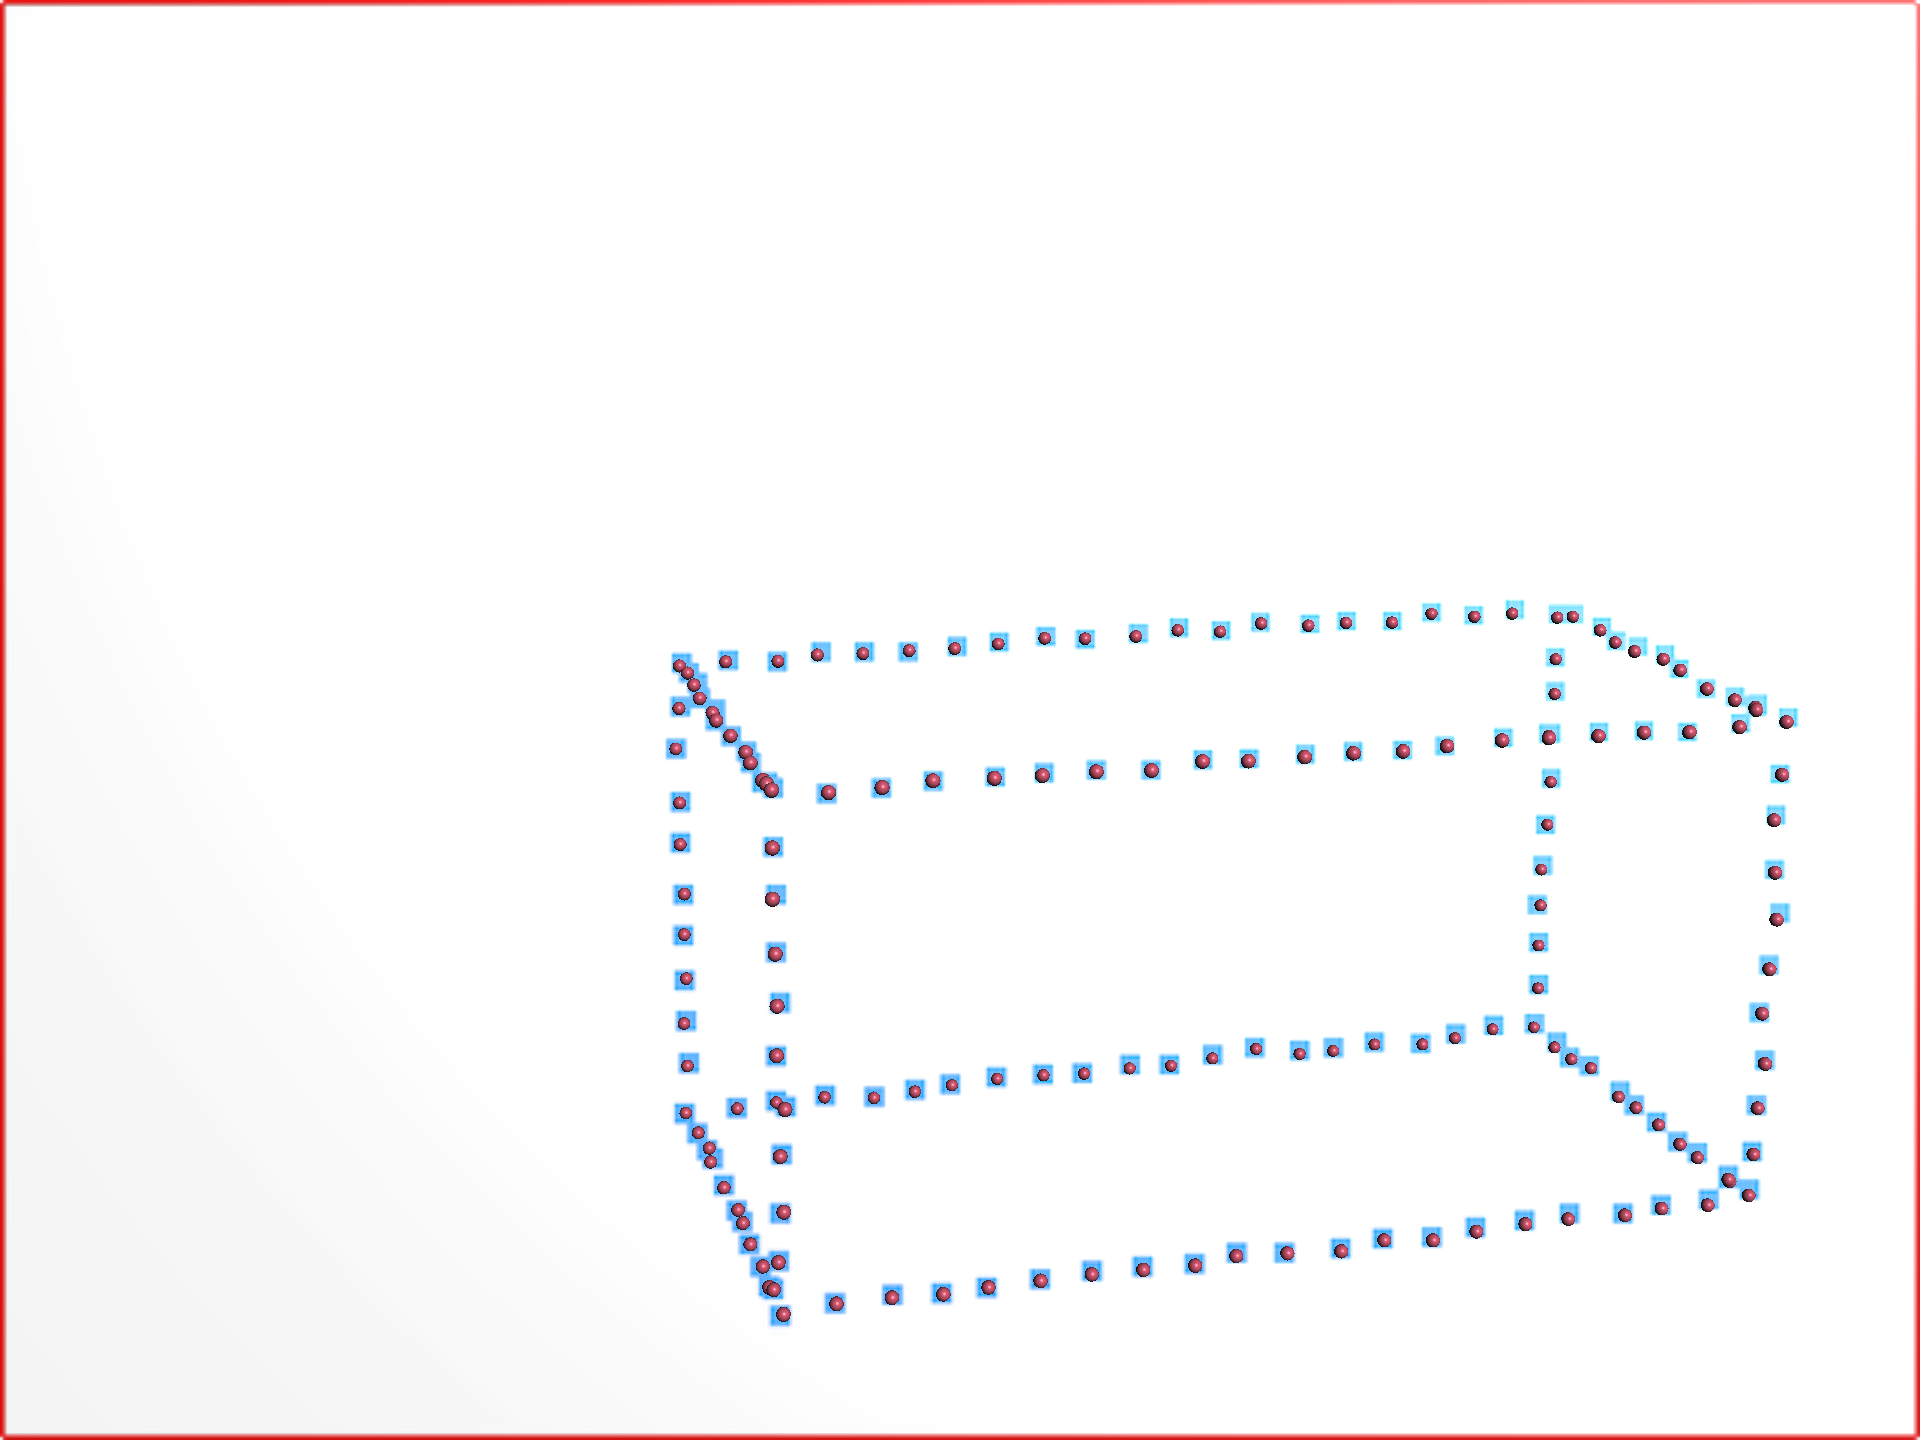
\includegraphics[width=0.9\linewidth]{Images/triangulation_final.png}
\end{subfigure}
\begin{subfigure}{0.55\textwidth}
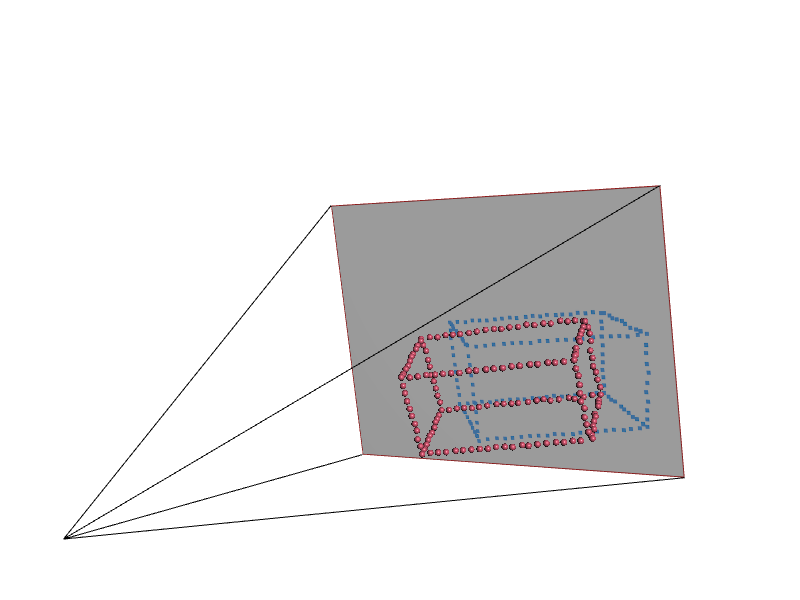
\includegraphics[width=0.9\linewidth]{Images/final_angle.png}
\end{subfigure}}
\caption{Reconstructed 3-D points with default camera parameters}
\label{fig:standard}
\end{figure}

\section{Effects of inaccuracies camera Parameters}
The methodology assumes the intrinsic camera parameters in $K$ to be known. If these are not accurate the quality of the projection will suffer. Given the accurate camera parameters we obtain an RMSE of $1.19$ pixels. Changing the focal lengths $f_x$ and $f_y$ downwards by 5\% actually decreases it to $1.08$, changing it upwards by the same percentage increases it to $1.42$. Overestimating the center of the image ($c_x,c_y)$ by 40 pixels increases it to $1.37$. Setting a skew parameter ($s$) of 10 yields an RMSE of $1.18$, again slightly lower.

Larger changes do result in larger RMSE, a skew parameter of 500 yields a RMSE of 8.89. A 20\% upwards adjustment of the focal length brings it up to 2.53. A similar adjustment of the image center by 100 pixels brings it to 3.37. Adjusting only one of the focal lengths by 20\% gives a far higher 18.96 pixel RMSE

Visually the dual focal length change gives a fairly similar result to the correct one, whereas the camera center change primarily shifts the position of the reconstructed points. Having only one focal length increase squishes the points together along that axis, whereas the box get predictably skewed for a high skew factor. These scenarios are depicted in Figure \ref{fig:changed_params}.

\begin{figure}[h]
\centering
\makebox[0pt]{
\begin{subfigure}{0.55\textwidth}
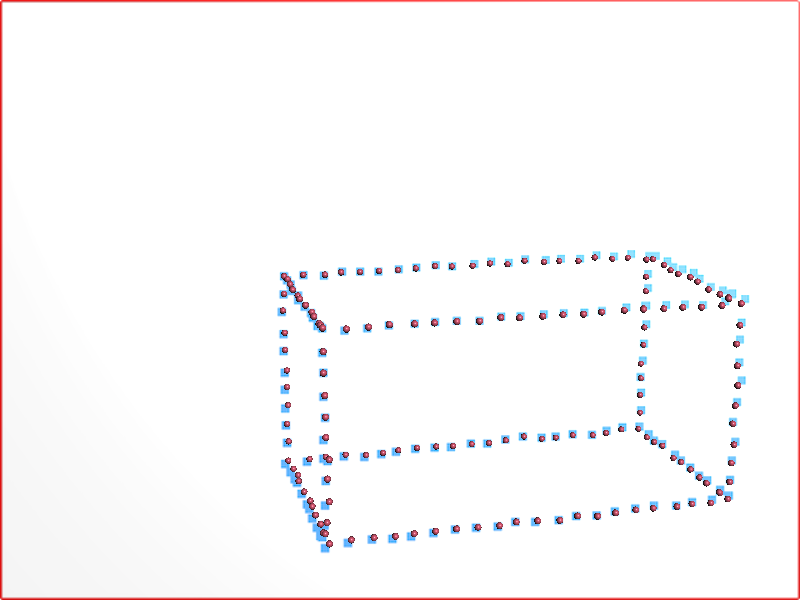
\includegraphics[width=0.9\linewidth]{Images/focal_changed.png}
\subcaption{Result with focal lengths increased by 20\%}
\end{subfigure}
\begin{subfigure}{0.55\textwidth}
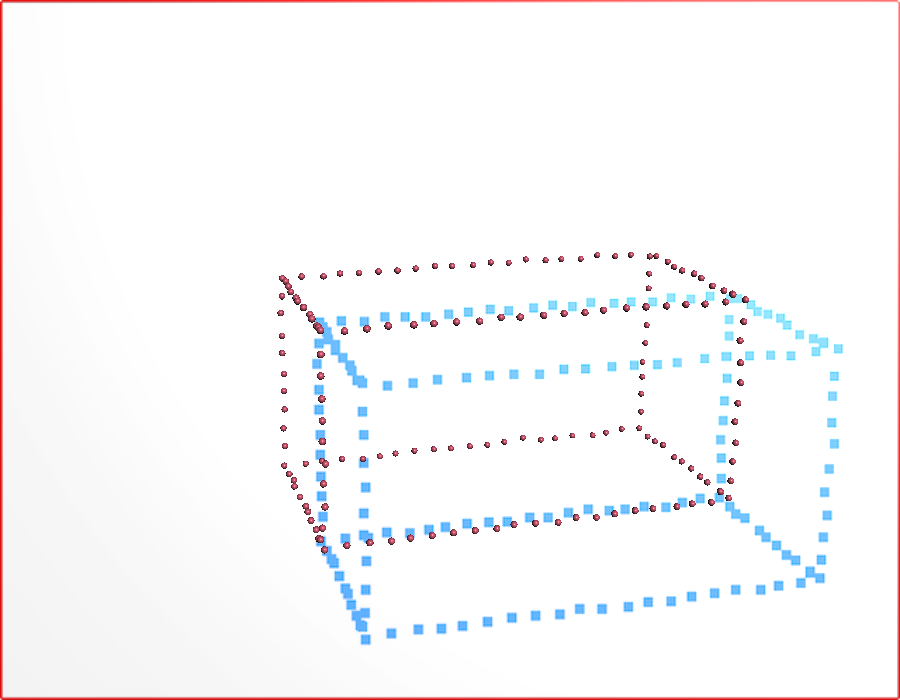
\includegraphics[width=0.9\linewidth]{Images/center_shift.png}
\subcaption{Result with image center coordinates increased by 40}
\end{subfigure}}\\
\makebox[0pt]{
\begin{subfigure}{0.55\textwidth}
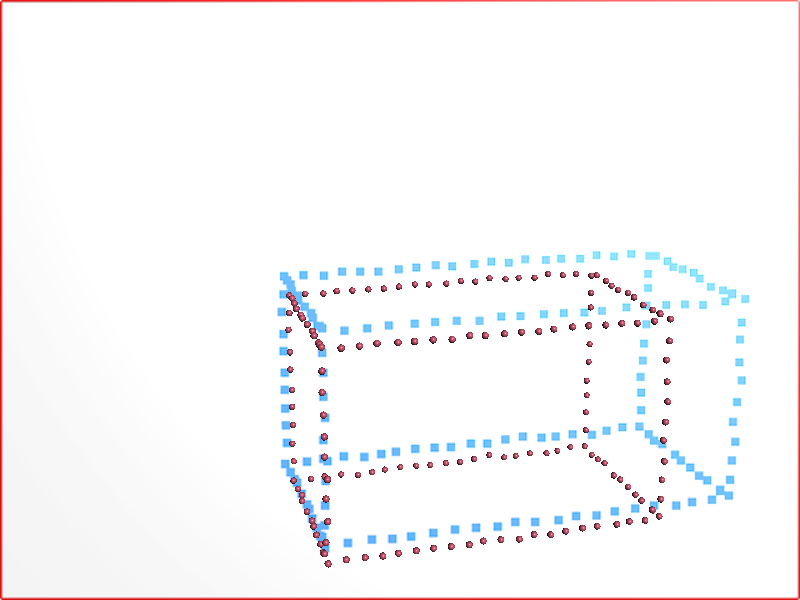
\includegraphics[width=0.9\linewidth]{Images/focal_change_1.png}
\subcaption{Result with only the focal length in $x$ increased by 20\%}
\end{subfigure}
\begin{subfigure}{0.55\textwidth}
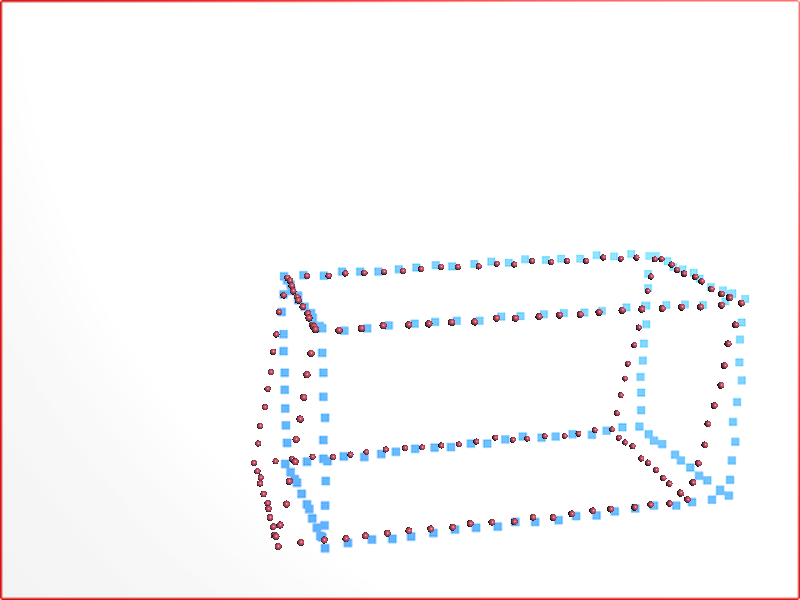
\includegraphics[width=0.9\linewidth]{Images/skewed.png}
\subcaption{Result with a skew factor of 200}
\end{subfigure}}
\caption{Resulting reconstructed points with changed parameters}
\label{fig:changed_params}
\end{figure}


\subsection{Possible improvements}
Adding additional views with accurate intrinsic camera parameters and accurate matching of points can lead to an improved accuracy for the points.

Given the camera intrinsics and image matching are both accurate, possible improvements can be established using Bundle Adjustment in order to minimize the total reprojection error. There we fit for both the camera extrinsic parameters and 3D points at the same time, whereas we assume the fitted extrinsic parameters to be perfect when fitting the 3D points in the approach in this report. The objective function to minimize here is given as:
\[
g(\mathbf{X}, \mathbf{R}, \mathbf{T}) = \sum_{i=1}^{m} \sum_{j=1}^{n} w_{ij} \cdot \left\| \mathbf{P}(\mathbf{x}_i, \mathbf{R}_j, \mathbf{t}_j) - \begin{bmatrix} u_{i,j} \\ v_{i,j} \end{bmatrix} \right\|^2
\]
with $w_{ij}$ an weight factor indicating whether point $i$ is visible in image $j$, $\mathbf{P}(\mathbf{x}_i, \mathbf{R}_j, \mathbf{t}_j)$ indicating the projected point  and the vector $\begin{bmatrix} u_{i,j} & v_{i,j} \end{bmatrix}^T$ being the observed image point.

% In real-world cases, accurate camera intrinsic parameters are extracted through geometric calibration using a known pattern, such as a checkerboard.
% By photographing this grid from different angles, we can compare the known 3-D points against their 2-D projections to derive the camera's focal length, principal point, and skew.

\subsubsection{Feedback and Implementation}
Group 3 reviewed our code, and their main feedback focused on improving the code formatting and the order of execution. Additionally, their suggestions on determining the correct camera pose helped us simplify the implementation, avoiding the need to overload everything into a single loop or use of complex array of pointers to matrices.

\section{Experiment}
Link to \href{https://github.com/Jcsegertudelft/Geo1016Assignment2}{GitHub project repository}.



\section{Work distribution}

\begin{table}[H]
    \centering 
    \caption{Division of the Tasks}
    \vspace{5pt}
    \begin{tabular}{@{} p{0.3\textwidth} p{0.3\textwidth} p{0.3\textwidth} @{}}
        \toprule
        \textbf{Job Segers (40\%)} & \textbf{Niranjan Pradeep (30\%)} & \textbf{Akhil Veeranki (30\%)} \\ 
        
        \midrule
            Estimation of Fundamental matrix & Candidate Poses \& Correct relative Pose & Linear triangulation of 3D Points \\
    Calculation of possible $R$ and $\mathbf{t}$ &Error Calculation & Report Section 1.1 \\
    Non-linear optimization & Feedback and Implementation & \\
    Report sections 1.1, 1.3, 1.4, 3 & 1.2, 3.1 & \\
        \bottomrule
    \end{tabular}
\end{table}


\end{document}